\chapter{仮想環境を使用したクラスタリング動作の検証}
\label{chap:fourth}

\section{緒言}
移行先のクラスタを構成するノードを増設する方法が不明であったので, 本章で検討する. 4.4節では2ノードで動作しているクラスタを3ノードにする. 4.5節では3ノードで動作しているクラスタに1ノード追加する. 本章では効率よく検討するためにDockerによる仮想環境を使用した.

\section{Dockerとは}
Dockerは, 軽量で独立したコンテナ型仮想環境用のプラットフォームである\cite {4}.

従来の仮想化では, VMWare\cite {5}などの仮想化ソフトウェアを用いて, ホストOS上にゲストOSを構築していた.
しかし, DockerはホストOS上にゲストOSなしで独立したコンテナ型の仮想環境として構築される.
Dockerコンテナは, Docker Engine上で動作する. Docker Engineはコンテナの立ち上げ, 停止, 削除といった操作を行う.

本論文では, Dockerイメージの形式で供給されているElasticsearchを使用したため, 以降で述べる動作する/しないの判定が素早くできた.

\begin{figure}[H]
  \begin{center}
    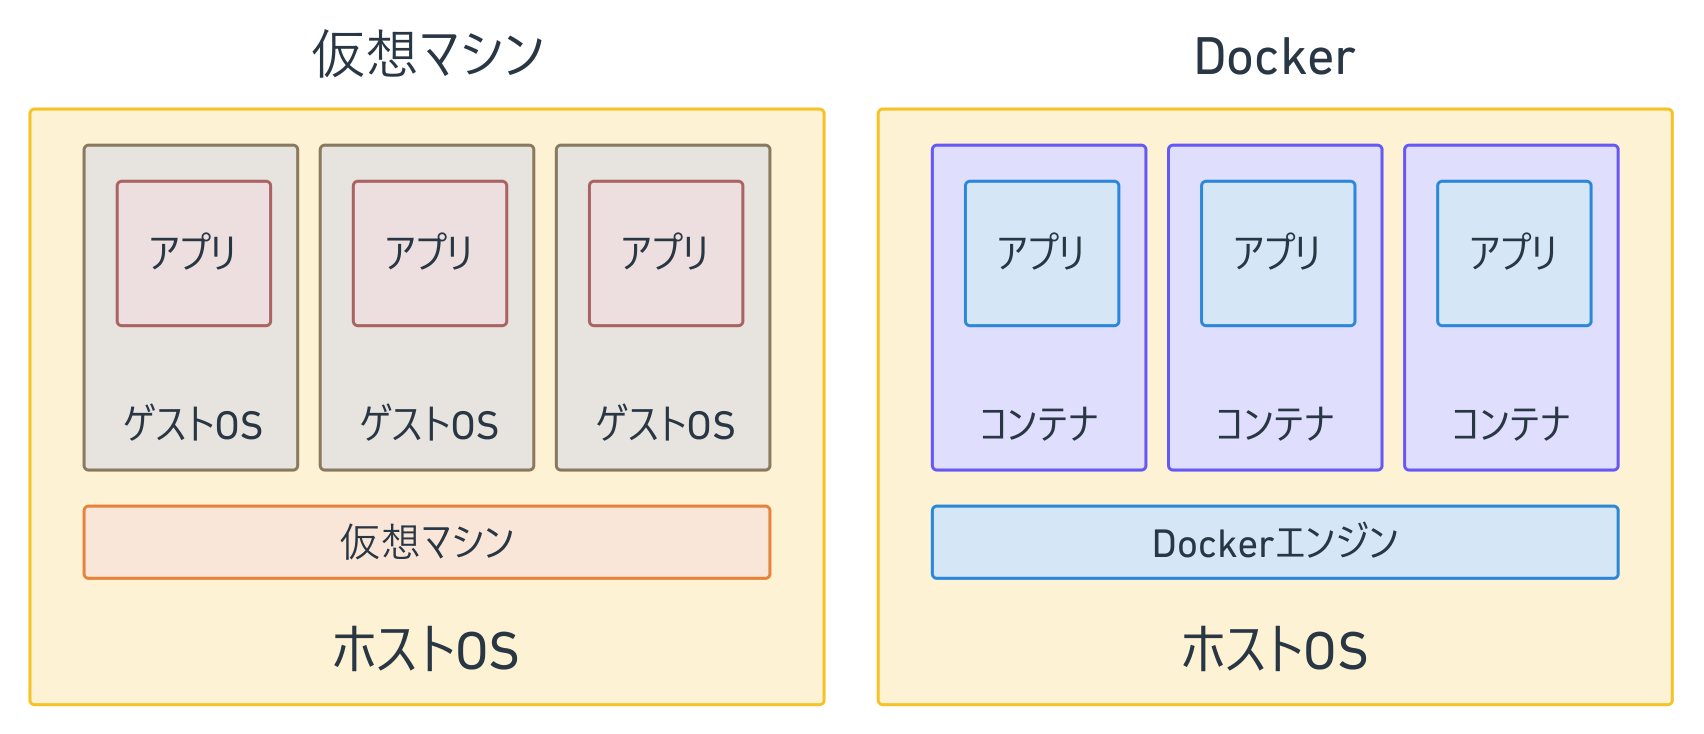
\includegraphics[width=140mm]{sotu/figure/docker-vmware.png}
    \caption{仮想マシンとDockerの違い}
    \label{4-p1}
  \end{center}
\end{figure}

\subsection{コンテナとは}

コンテナは, アプリケーションとそのすべての依存関係(ライブラリ, 実行環境など)をカプセル化した軽量な実行単位である.
Dockerの場合, コンテナの作成にはDockerイメージが必要となる.

\subsection{Dockerイメージとは}

Dockerイメージとは, Dockerコンテナを作成するためのテンプレートであり, Dockerイメージの中には, Docker コンテナの実行に必要な Linux ファイルシステムとメタ情報を含む.

Linux ファイルシステムというのは,  / ディレクトリ以下の /etc /bin /sbin /usr などのディレクトリ階層およびファイルである. 

Docker では, コンテナとして動かしたいアプリケーションが必要とする, 最小限のファイルを Docker イメージの中に入れる. 

さらに, そのアプリケーションを動かすために必要なデフォルトのコマンドや引数の指定, 外に公開するポート番号の情報などの情報がある. これらをメタ情報として, 同じく Docker イメージの中に入れられる 

DockerイメージはDocker Hubやその他のレジストリで共有されており, これらのサービスから取得することが可能である.

今回はElasticsearchの開発元であるElastic社が提供しているElasticsearchのDockerイメージを使って検証を行う.

\begin{figure}[H]
  \begin{center}
    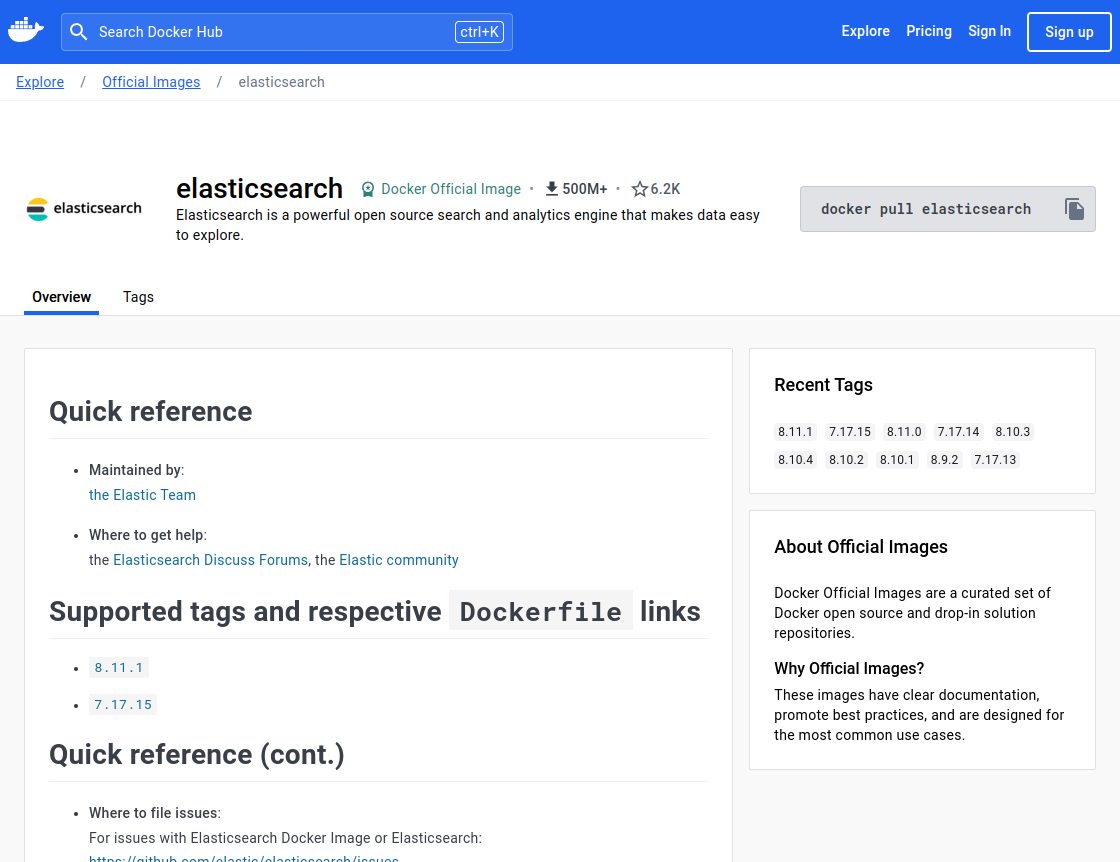
\includegraphics[width=120mm]{sotu/figure/elasticsearch-image.png}
    \caption{ElasticsearchのDockerイメージ}
    \label{4-p2}
  \end{center}
\end{figure}

\section{Docker Composeとは}
Docker Composeは, 複数のコンテナを定義し, 実行するためのツールである. これはYAMLファイルを使用して設定され, 複数のコンテナで協調して動作するアプリケーションの開発を単純化する.

\section{バージョンの異なるElasticsearchノードを用いたクラスタ構築の可否の検証}
\subsection{全て同じバージョンのElasticsearchを使用したクラスタ構成 (全ノード バージョン 7.17.9)}

図 \ref{4-p3}に, 7.17.9バージョンのElasticsearchのみを使用してクラスタを構築した時のdocker-compose.ymlを図で表現したものを示す.

\begin{figure}[H]
  \begin{center}
    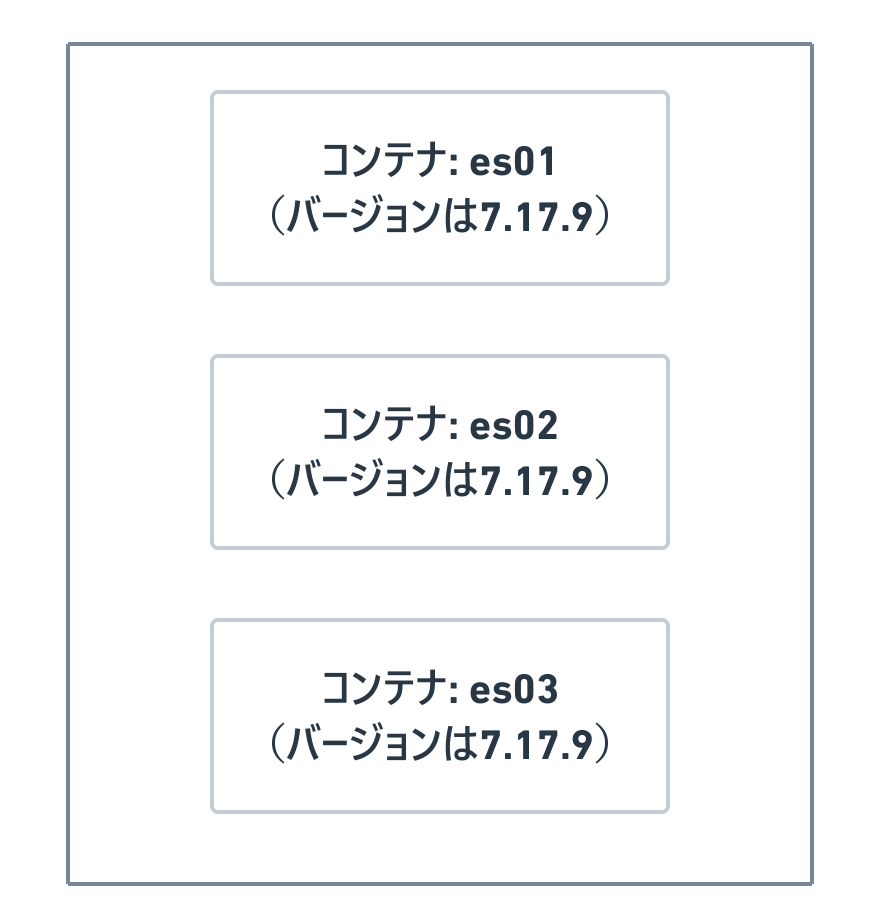
\includegraphics[width=110mm]{sotu/figure/all-7.19.9.png}
    \caption{docker-compose.ymlを図で表現したもの}
    \label{4-p3}
  \end{center}
\end{figure}

クラスタの起動には, docker compose up -dコマンドを使用する.

docker compose up -dコマンドを実行した後, curlコマンドを使用してクラスタに参加しているノードを一覧表示した結果をリスト \ref{4-sc1}に示す.

% \begin{figure}[H]
%   \begin{center}
%     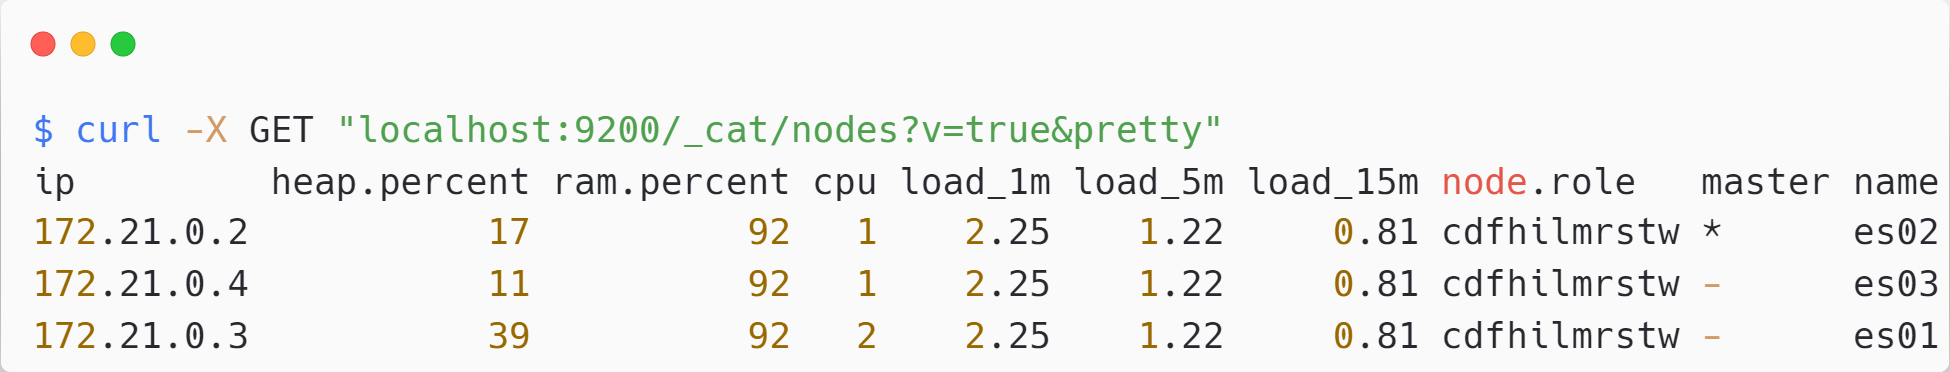
\includegraphics[width=140mm]{sotu/figure/curl-same.png}
%     \caption{クラスタに参加しているノードを一覧表示した結果}
%     \label{4-p4}
%   \end{center}
% \end{figure}
\begin{lstlisting}[language=bash, caption=クラスタに参加しているノードを一覧表示した結果, label=4-sc1]
  $ curl -X GET "localhost:9200/_cat/nodes?v=true&pretty"
  ip         heap.percent ram.percent cpu load_1m load_5m load_15m node.role   master name
  172.21.0.2           17          92   1    2.25    1.22     0.81 cdfhilmrstw *      es02
  172.21.0.4           11          92   1    2.25    1.22     0.81 cdfhilmrstw -      es03
  172.21.0.3           39          92   2    2.25    1.22     0.81 cdfhilmrstw -      es01
\end{lstlisting}

リスト \ref{4-sc1}より, 3つのノード(es01, es02, es03)すべてが正常にクラスタに参加できていることが確認できる.

\subsection{異なるバージョンのElasticsearchを使用したクラスタ構成 (2ノード バージョン 7.17.9, 1ノード バージョン 7.17.6)}

図 \ref{4-p3}で示されたdocker-compose.ymlにおいて, es03のコンテナで使用されるDockerイメージを変更して, Elasticsearchのバージョンを7.17.9から7.17.6にダウングレードする.

図 \ref{4-p5}に変更後のdocker-compose.ymlを図で表現したものを示す.

\begin{figure}[H]
  \begin{center}
    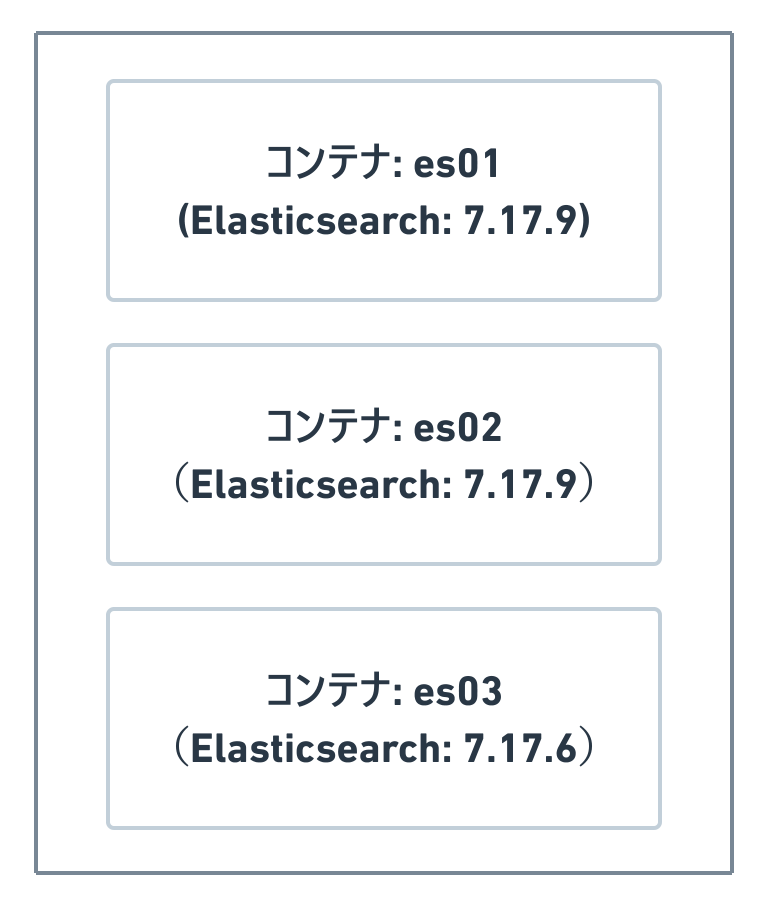
\includegraphics[width=110mm]{sotu/figure/2-7.19.9-and-1-7.17.6.png}
    \caption{変更後のdocker-compose.ymlを図で表現したもの}
    \label{4-p5}
  \end{center}
\end{figure}

変更後, docker compose up -dコマンドを実行してクラスタを起動する.

クラスタの起動後, curlコマンドを使用してクラスタに参加しているノードを一覧表示した結果をリスト \ref{4-sc2}に示す.

% \begin{figure}[H]
%   \begin{center}
%     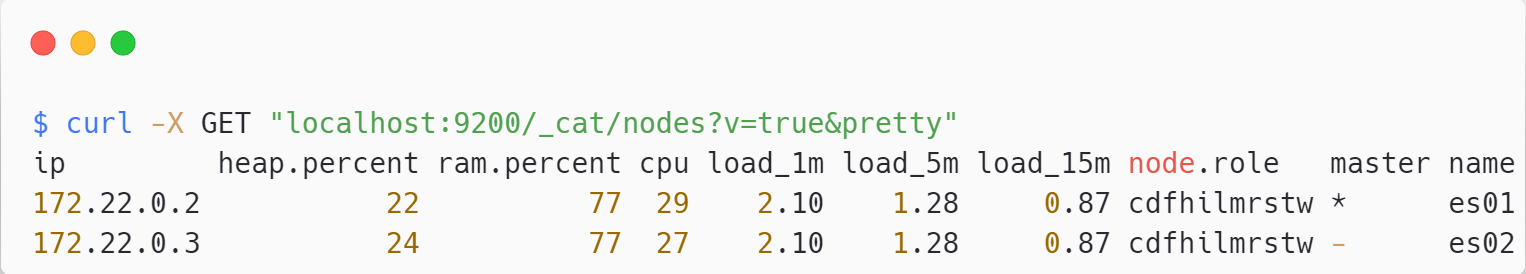
\includegraphics[width=140mm]{sotu/figure/curl-different.png}
%     \caption{クラスタに参加しているノードを一覧表示した結果}
%     \label{4-p6}
%   \end{center}
% \end{figure}
\begin{lstlisting}[language=bash, caption=クラスタに参加しているノードを一覧表示した結果, label=4-sc2]
  $ curl -X GET "localhost:9200/_cat/nodes?v=true&pretty"
  ip         heap.percent ram.percent cpu load_1m load_5m load_15m node.role   master name
  172.22.0.2           22          77  29    2.10    1.28     0.87 cdfhilmrstw *      es01
  172.22.0.3           24          77  27    2.10    1.28     0.87 cdfhilmrstw -      es02
\end{lstlisting}

リスト \ref{4-sc2}より, Elasticsearchのバージョンが7.17.9である2つのノード(es01, es02)のみがクラスタに参加できていることが確認できる.

es03のコンテナでElasticsearchの起動を試みた時に出力されたログを確認したところ, リスト \ref{4-sc3}に示すエラーログを出力して起動に失敗していた.

% \begin{figure}[H]
%   \begin{center}
%     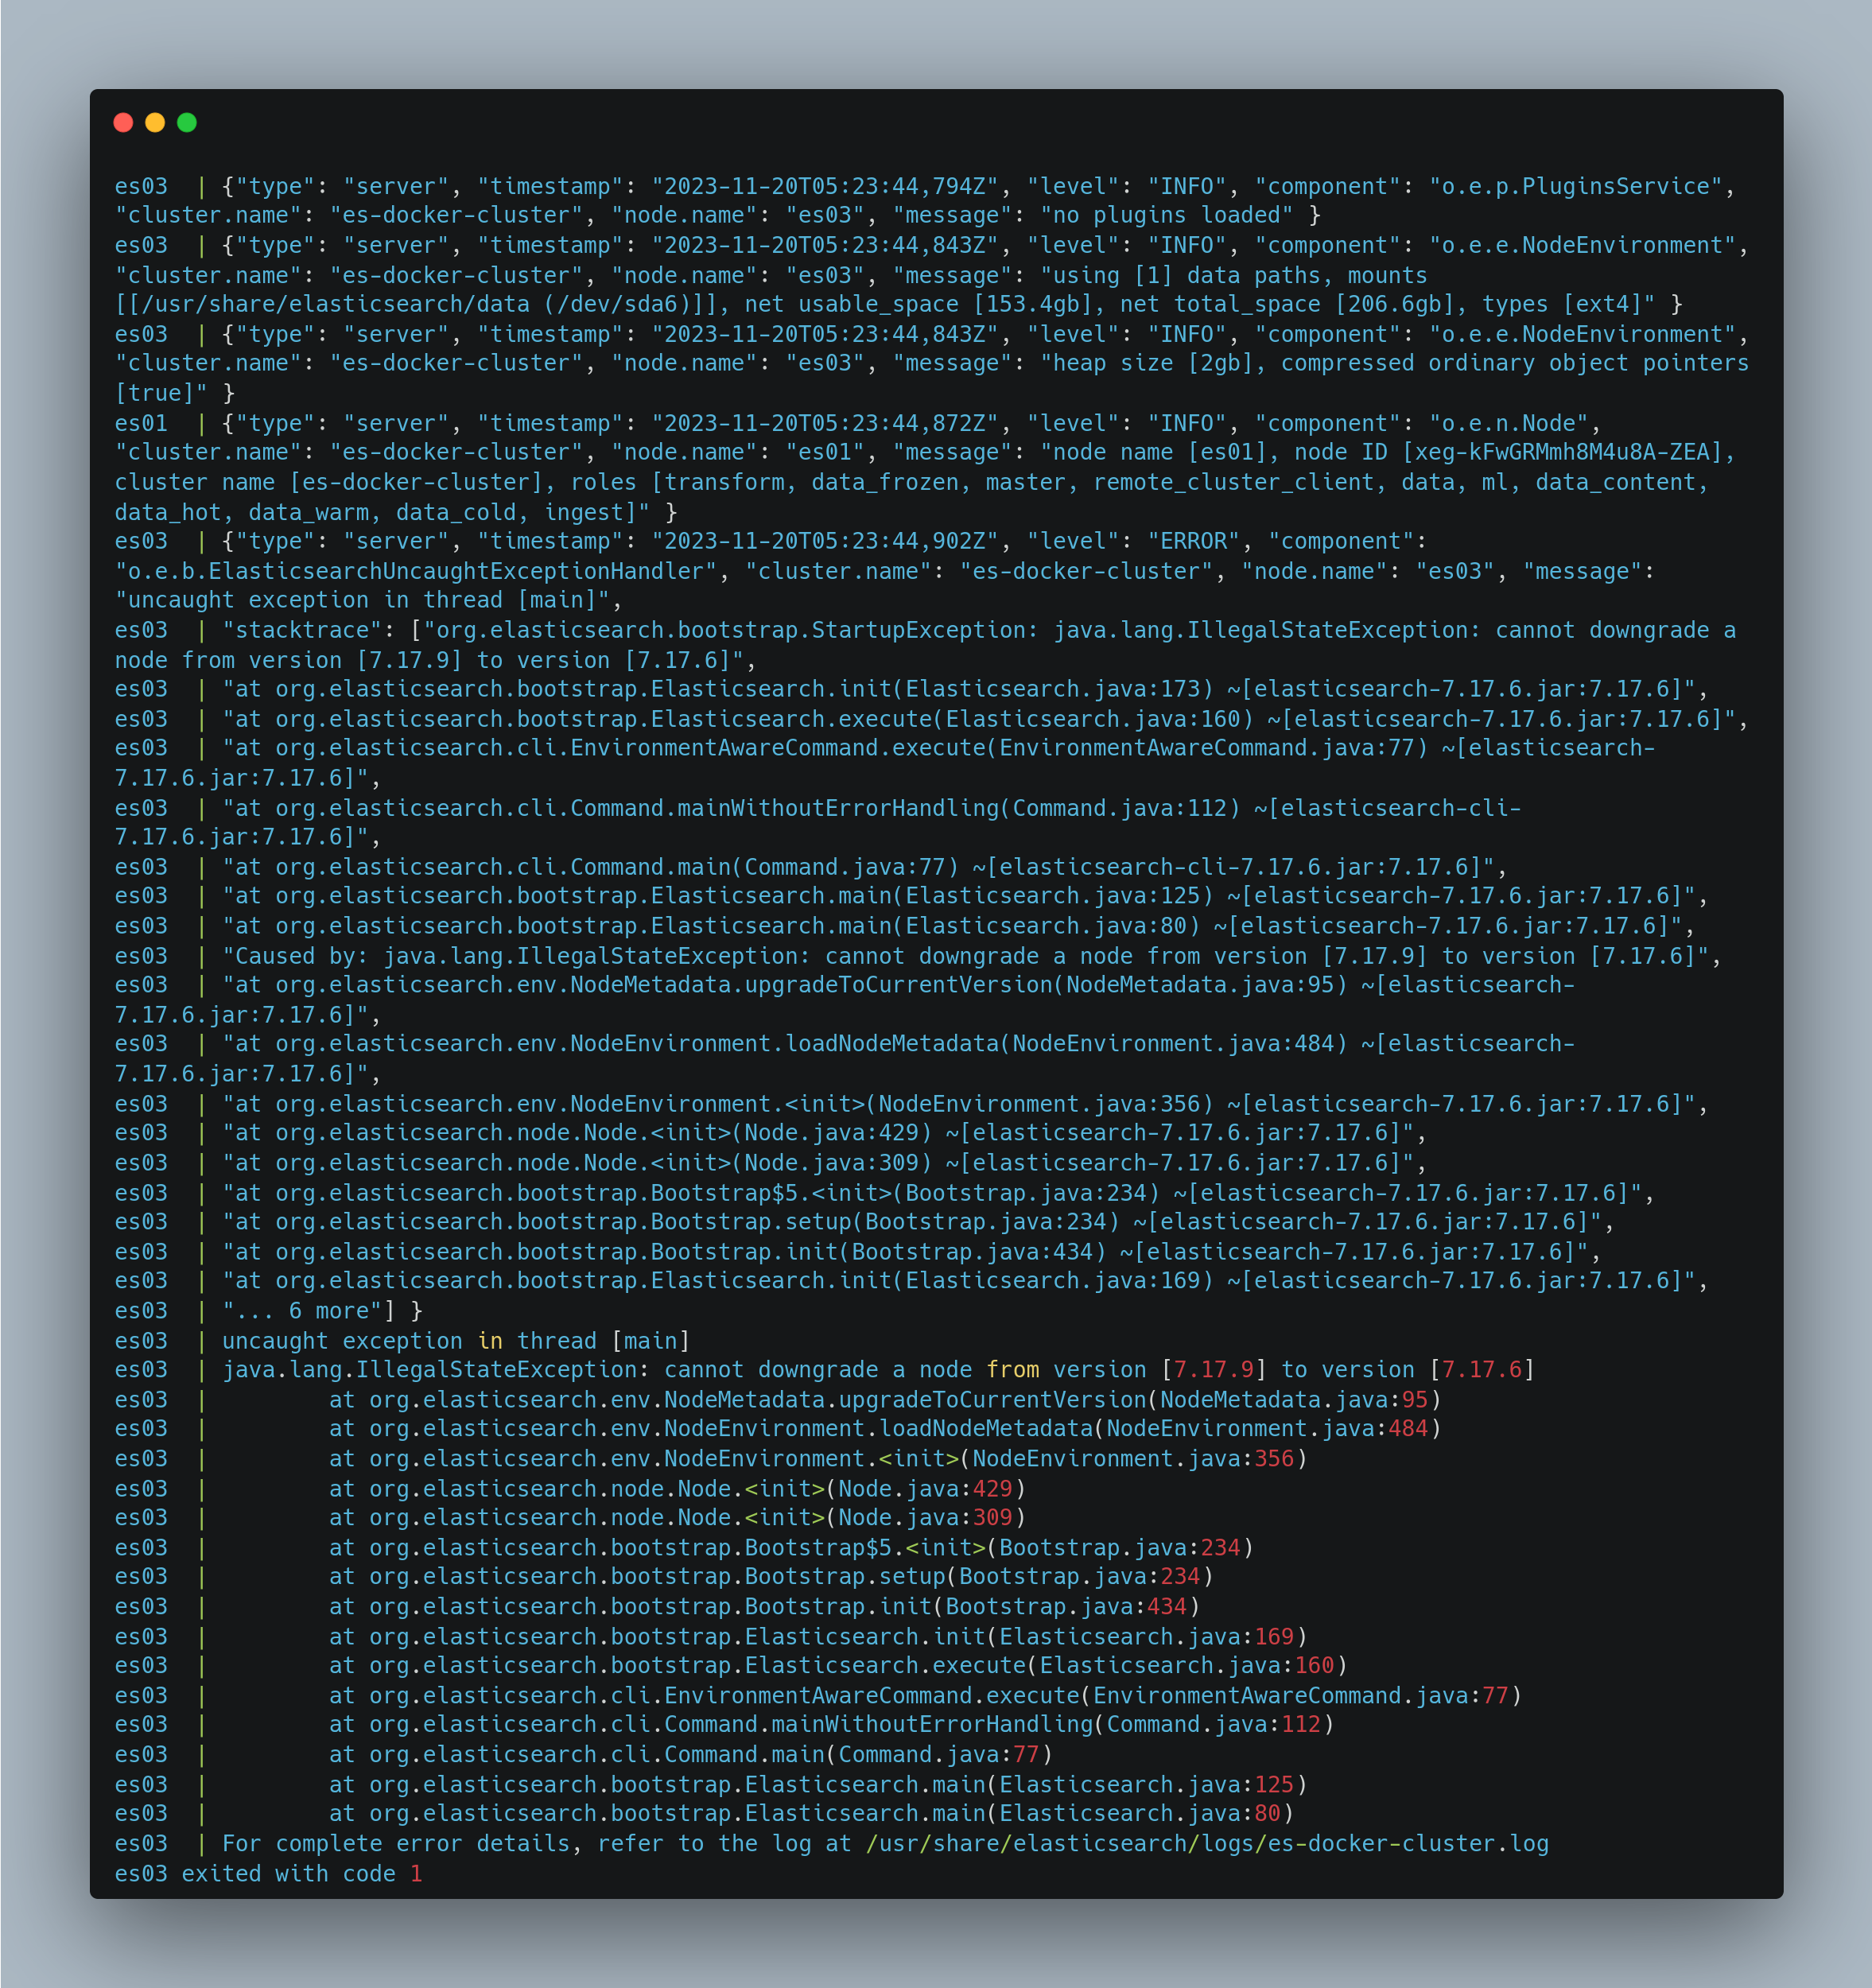
\includegraphics[width=140mm]{sotu/figure/log.png}
%     \caption{es03のログ}
%     \label{4-p7}
%   \end{center}
% \end{figure}
\begin{lstlisting}[language=bash, caption=es03のログ, label=4-sc3]
  es03  | java.lang.IllegalStateException: cannot downgrade a
  node from version [7.17.9] to version [7.17.6]
\end{lstlisting}

\section{既存Elasticsearchノードの異なるクラスタへの参加の可否の検証}
クラスタ構築において, 既に稼働しているElasticsearchノードを新たなノードとして異なるクラスタへ参加できるか, Dockerによる仮想環境を用いて検証した.

\subsection{単一ノードで稼働するクラスタAの構築}

まず, docker-composeを用いて単一ノード(コンテナ名はes04)でクラスタを構築する. 以後このクラスタをクラスタAと呼ぶ.

図 \ref{4-p8}にクラスタAを構築する際に使用したdocker-compose.ymlを図で表現したものを示す.

\begin{figure}[H]
  \begin{center}
    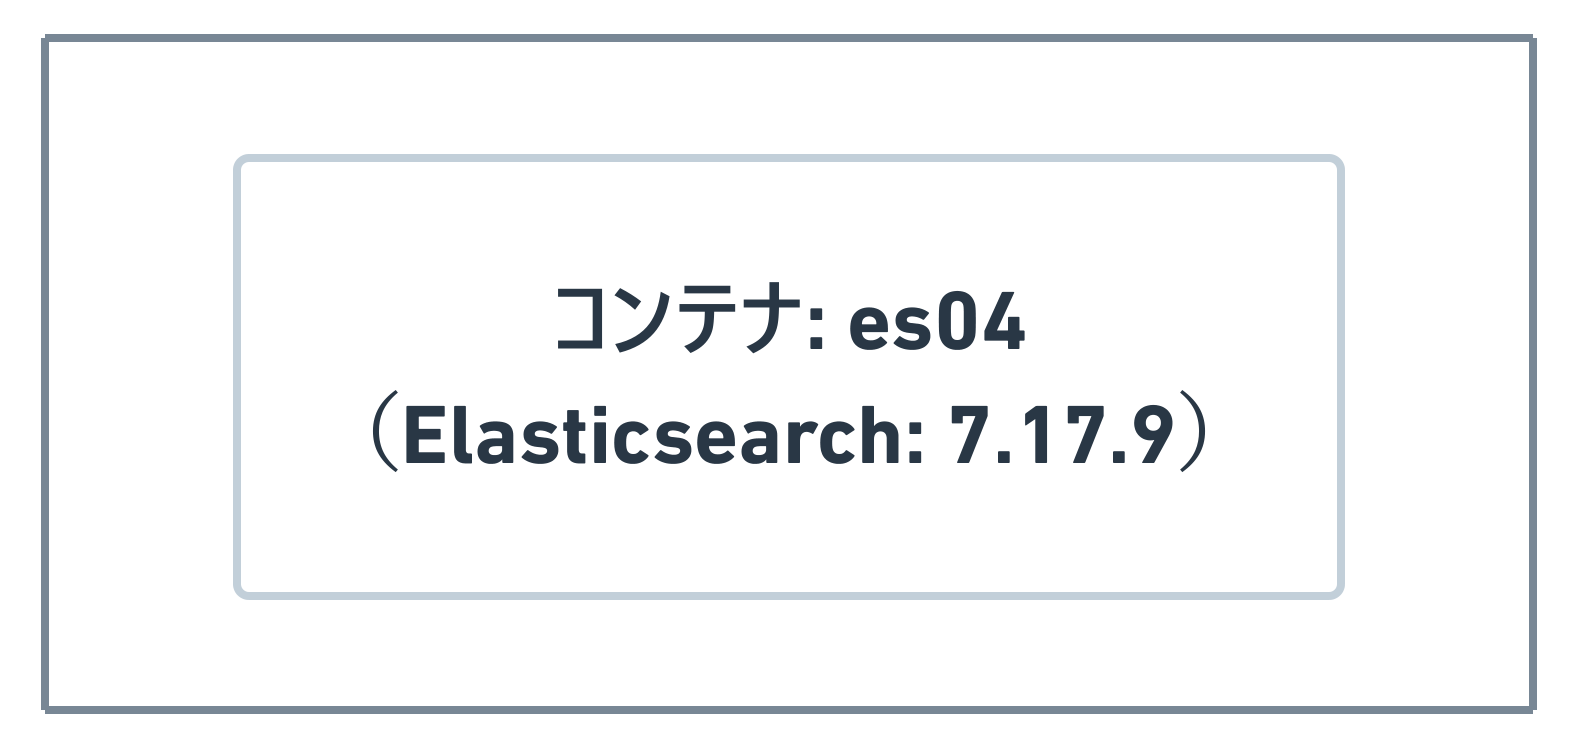
\includegraphics[width=100mm]{sotu/figure/1-7.17.9.png}
    \caption{クラスタAを構築する際に使用したdocker-compose.ymlを図で表現したもの}
    \label{4-p8}
  \end{center}
\end{figure}

docker-composeを用いてクラスタAを起動した後, クラスタの情報について問い合わせた結果をリスト \ref{4-sc4}に示す.

% \begin{figure}[H]
%   \begin{center}
%     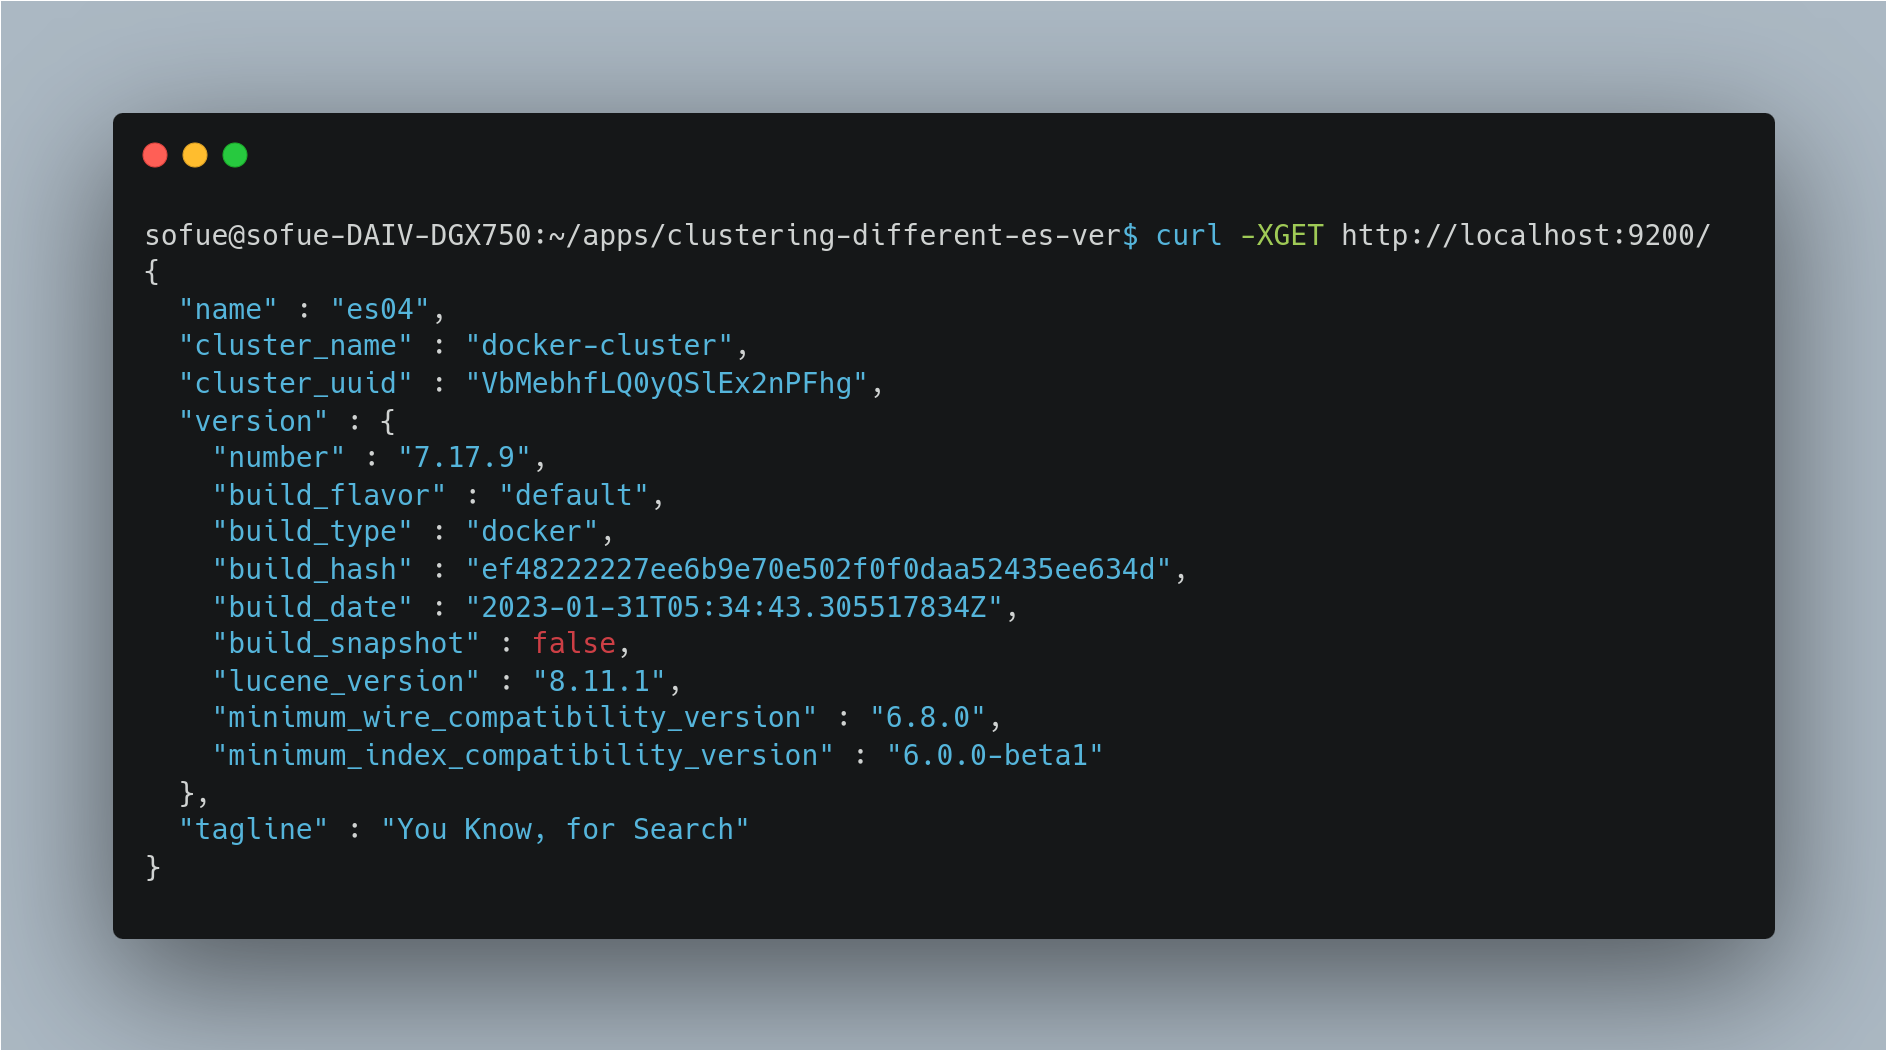
\includegraphics[width=140mm]{sotu/figure/es04-cluster.png}
%     \caption{クラスタの情報について問い合わせた結果}
%     \label{4-p9}
%   \end{center}
% \end{figure}
\begin{lstlisting}[language=bash, caption=クラスタAの情報について問い合わせた結果, label=4-sc4, breaklines=false]
  $ curl -XGET http://localhost:9200/
  {
    "name" : "es04",
    "cluster_name" : "docker-cluster",
    "cluster_uuid" : "NCg_UaW0Q6KTakJG5HJrHg",
    "version" : {
      "number" : "7.17.9",
      "build_flavor" : "default",
      "build_type" : "docker",
      "build_hash" : "ef48222227ee6b9e70e502f0f0daa52435ee634d",
      "build_date" : "2023-01-31T05:34:43.305517834Z",
      "build_snapshot" : false,
      "lucene_version" : "8.11.1",
      "minimum_wire_compatibility_version" : "6.8.0",
      "minimum_index_compatibility_version" : "6.0.0-beta1"
    },
    "tagline" : "You Know, for Search"
  }
\end{lstlisting}

クラスタの情報について問い合わせた後, Dockerコンテナを停止してノードをシャットダウンした.

\subsection{3ノードで稼働するクラスタBの構築}

次に, クラスタAの構築に使用したノードとは別の3ノード(コンテナ名はそれぞれes01, es02, es03)でクラスタを構築する. 以後このクラスタをクラスタBと呼ぶ.

図 \ref{4-p10}にクラスタBの構築の際に使用したdocker-compose.ymlを図で表現したものを示す.

\begin{figure}[H]
  \begin{center}
    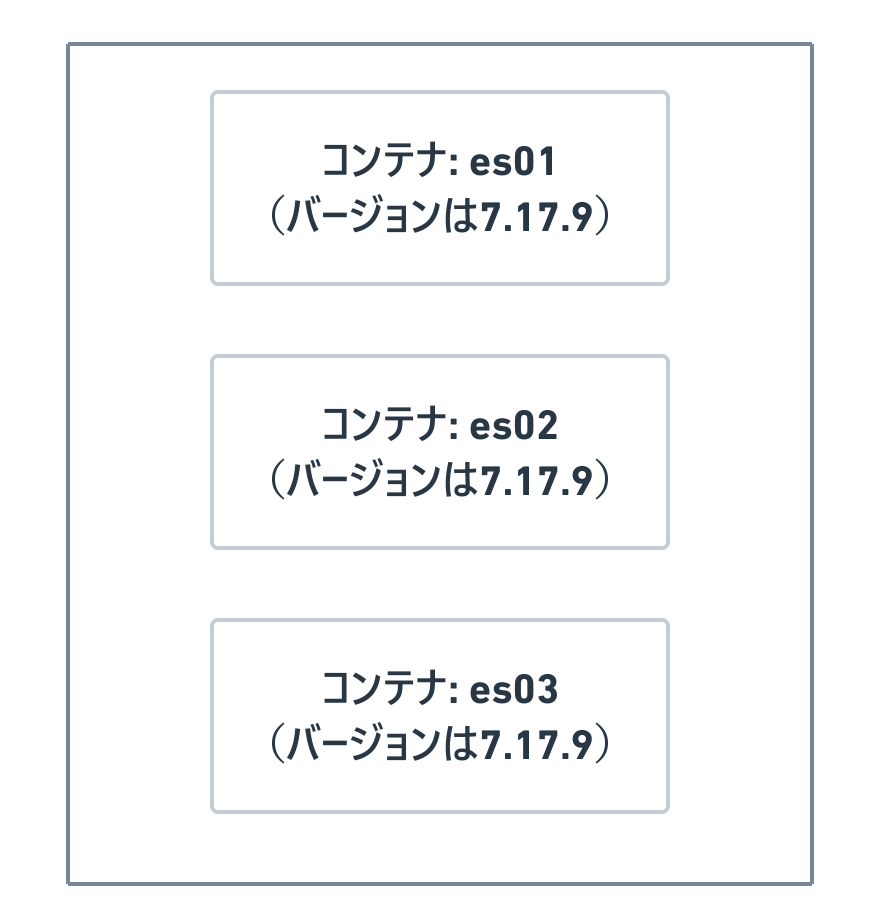
\includegraphics[width=110mm]{sotu/figure/all-7.19.9.png}
    \caption{クラスタBを構築する際に使用したdocker-compose.ymlを図で表現したもの}
    \label{4-p10}
  \end{center}
\end{figure}

docker-composeを用いてクラスタBを起動した後, クラスタの情報について問い合わせた結果をリスト \ref{4-sc5}に示す.

% \begin{figure}[H]
%   \begin{center}
%     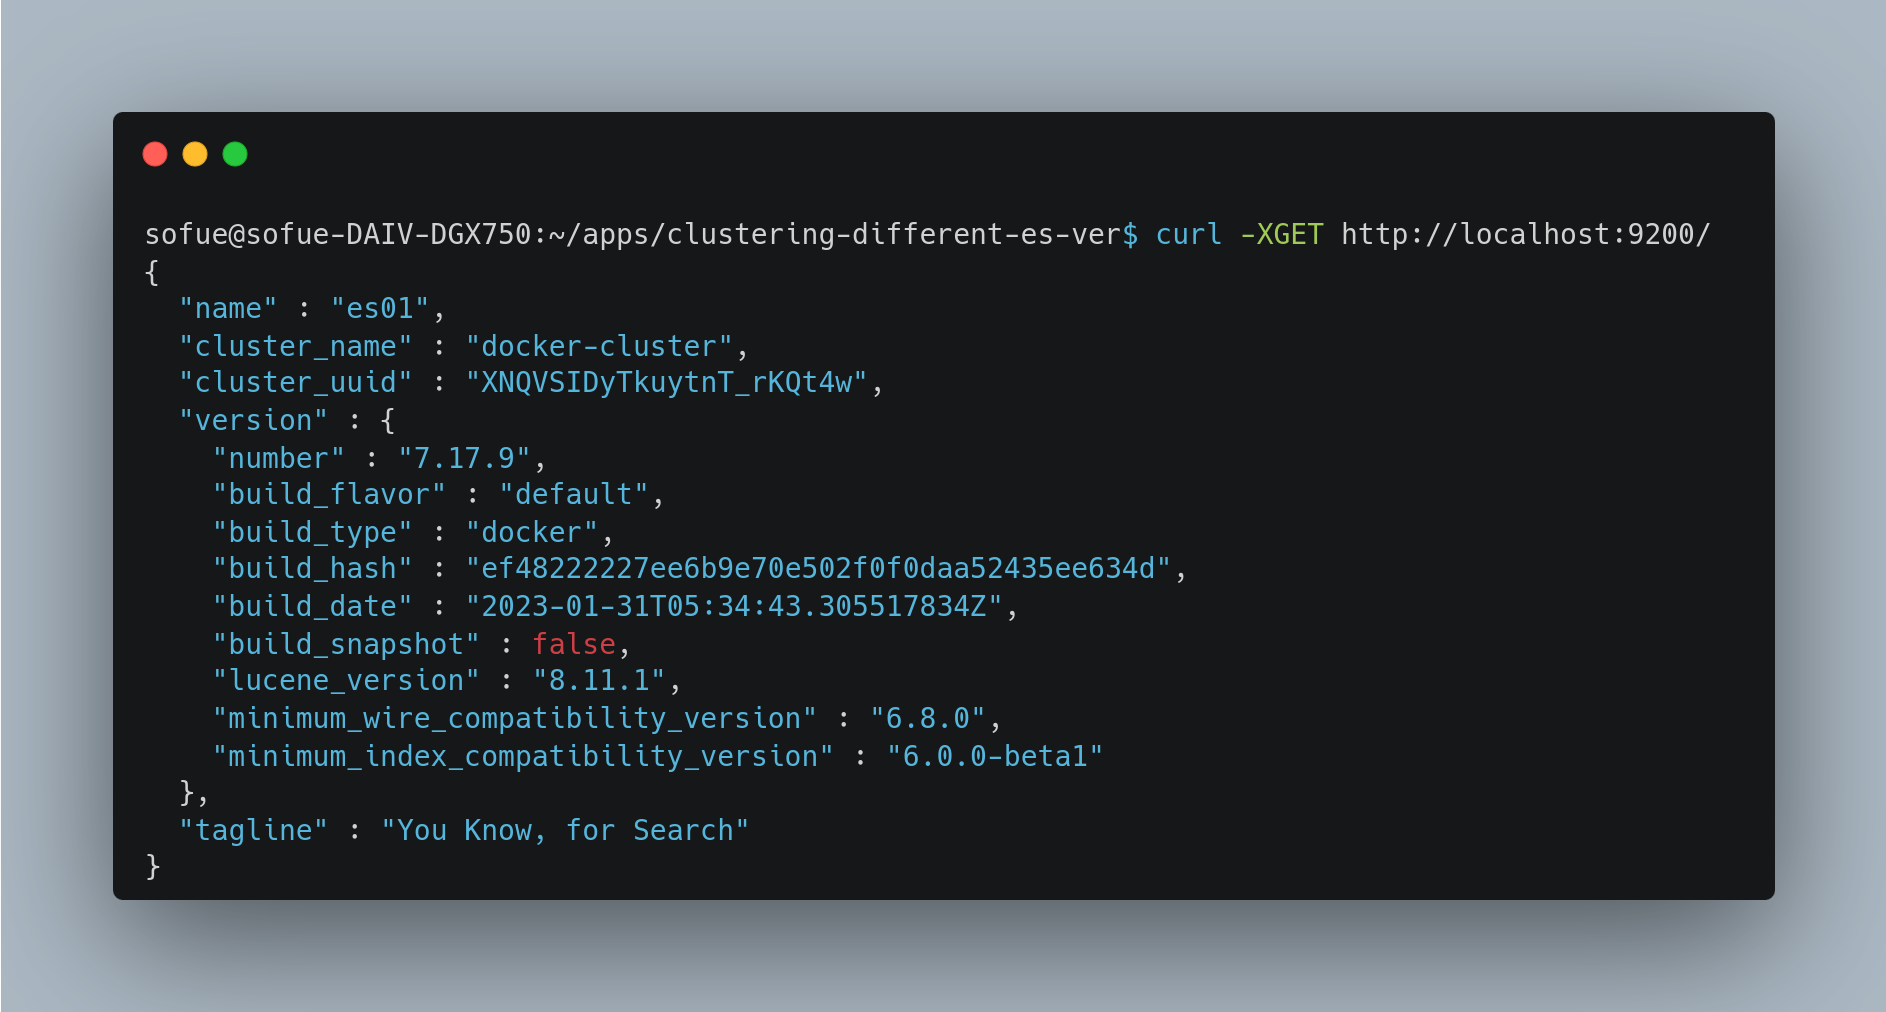
\includegraphics[width=140mm]{sotu/figure/3nodes-cluster.png}
%     \caption{クラスタの情報について問い合わせた結果}
%     \label{4-p11}
%   \end{center}
% \end{figure}
\begin{lstlisting}[language=bash, caption=クラスタBの情報について問い合わせた結果, label=4-sc5, breaklines=false]
  $ curl -XGET http://localhost:9200/
  {
    "name" : "es01",
    "cluster_name" : "docker-cluster",
    "cluster_uuid" : "2A69V1hxSFCisgmIo1LB_A",
    "version" : {
      "number" : "7.17.9",
      "build_flavor" : "default",
      "build_type" : "docker",
      "build_hash" : "ef48222227ee6b9e70e502f0f0daa52435ee634d",
      "build_date" : "2023-01-31T05:34:43.305517834Z",
      "build_snapshot" : false,
      "lucene_version" : "8.11.1",
      "minimum_wire_compatibility_version" : "6.8.0",
      "minimum_index_compatibility_version" : "6.0.0-beta1"
    },
    "tagline" : "You Know, for Search"
  }
\end{lstlisting}

リスト \ref{4-sc4}とリスト \ref{4-sc5}を比較した結果, クラスタAとクラスタBはそれぞれ異なるクラスタIDを付与されたことが分かった.

クラスタBの起動後, クラスタに参加しているノードの一覧を取得した結果をリスト \ref{4-sc6}に示す.

% \begin{figure}[H]
%   \begin{center}
%     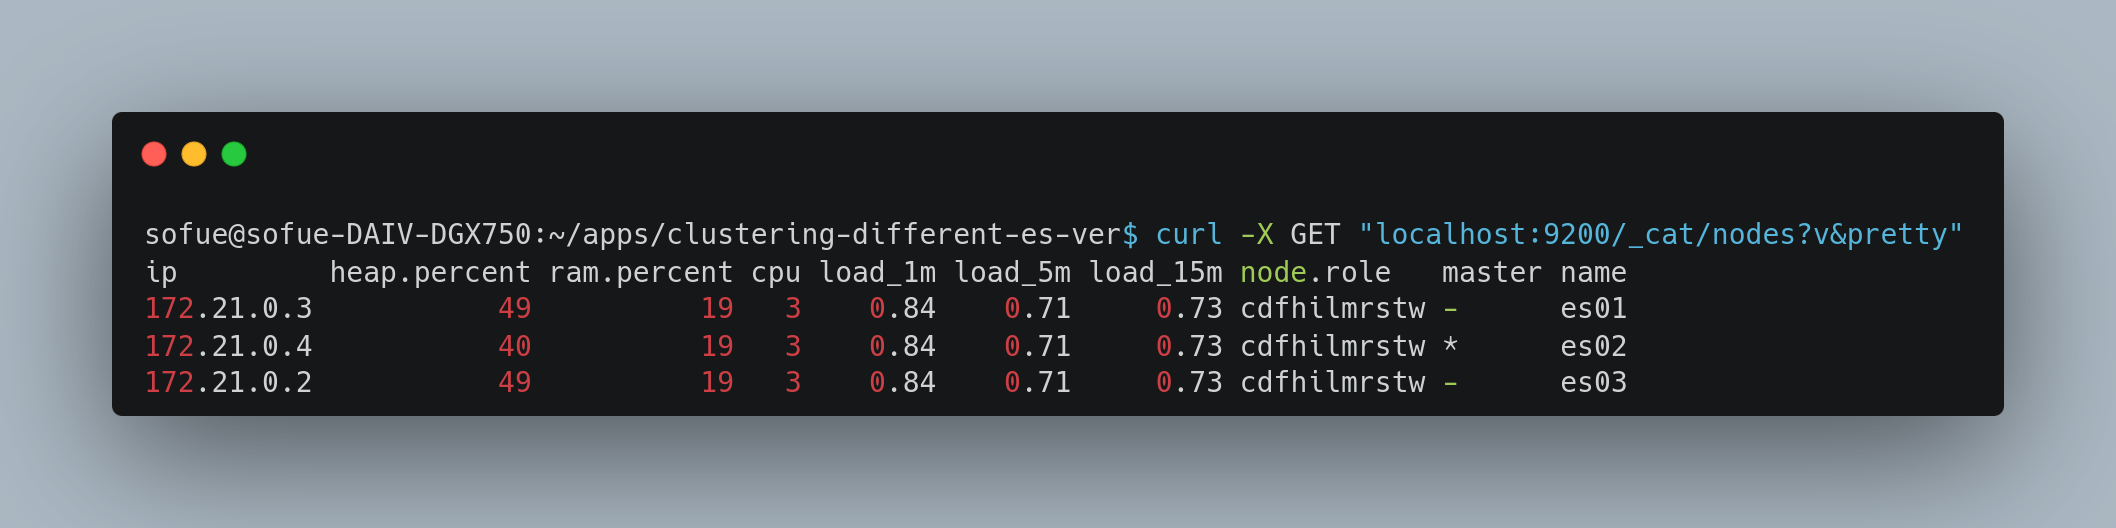
\includegraphics[width=140mm]{sotu/figure/3nodes-list.png}
%     \caption{クラスタに参加しているノード一覧}
%     \label{4-p12}
%   \end{center}
% \end{figure}
\begin{lstlisting}[language=bash, caption=クラスタBに参加しているノード一覧, label=4-sc6]
  $ curl -X GET 'localhost:9200/_cat/nodes?v&pretty'
  ip         heap.percent ram.percent cpu load_1m load_5m load_15m node.role   master name
  172.30.0.4           22          88  28    5.99    2.99     1.72 cdfhilmrstw -      es03
  172.30.0.3           17          88  29    5.99    2.99     1.72 cdfhilmrstw *      es02
  172.30.0.2           36          88  30    5.99    2.99     1.72 cdfhilmrstw -      es01
\end{lstlisting}

リスト \ref{4-sc6}より, es01, es02, es03ノードがクラスタBに参加できていることを確認した.

クラスタBに参加しているノードの一覧を取得した後, 全てのDockerコンテナを停止してノードを全てシャットダウンした.

\subsection{クラスタAに参加しているノードのクラスタBへの参加試行}

次に, 図 \ref{4-p10}のdocker-compose.ymlに対して, クラスタAのノード(es04コンテナ)を追加し, 合計4ノードでのクラスタBの起動を試みる.

図 \ref{4-p13}に, es04コンテナを含めた4ノードでクラスタBの起動を試みた際に使用したdocker-compose.ymlを図で表現したものを示す.

\begin{figure}[H]
  \begin{center}
    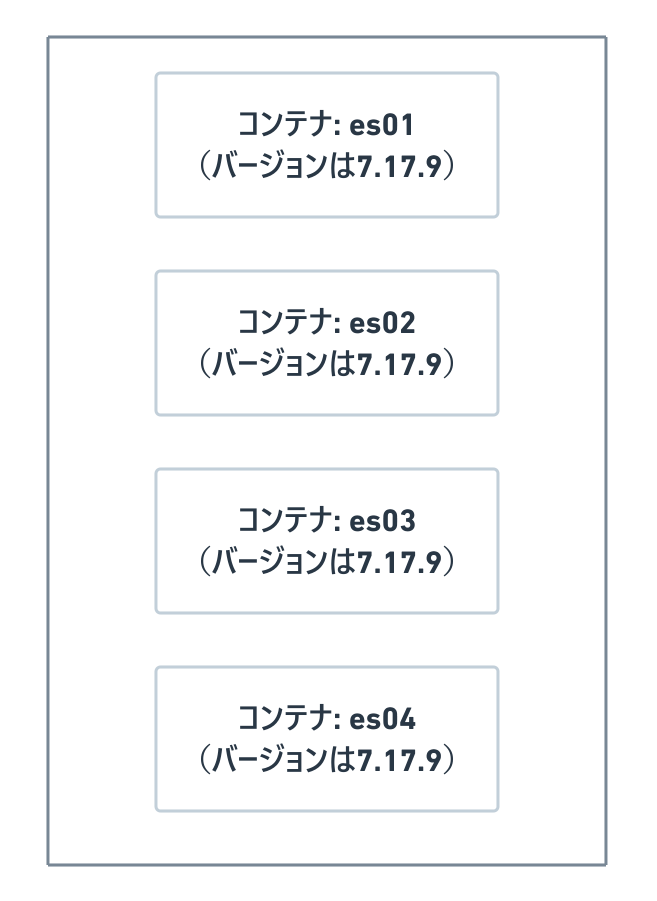
\includegraphics[width=110mm]{sotu/figure/4-7.17.9.png}
    \caption{es04コンテナを含めた4ノードでクラスタBの起動を試みた際に使用したdocker-compose.ymlを図で表現したもの}
    \label{4-p13}
  \end{center}
\end{figure}

クラスタBの起動後, クラスタに参加しているノードの一覧を取得した結果をリスト \ref{4-sc7}に示す.

% \begin{figure}[H]
%   \begin{center}
%     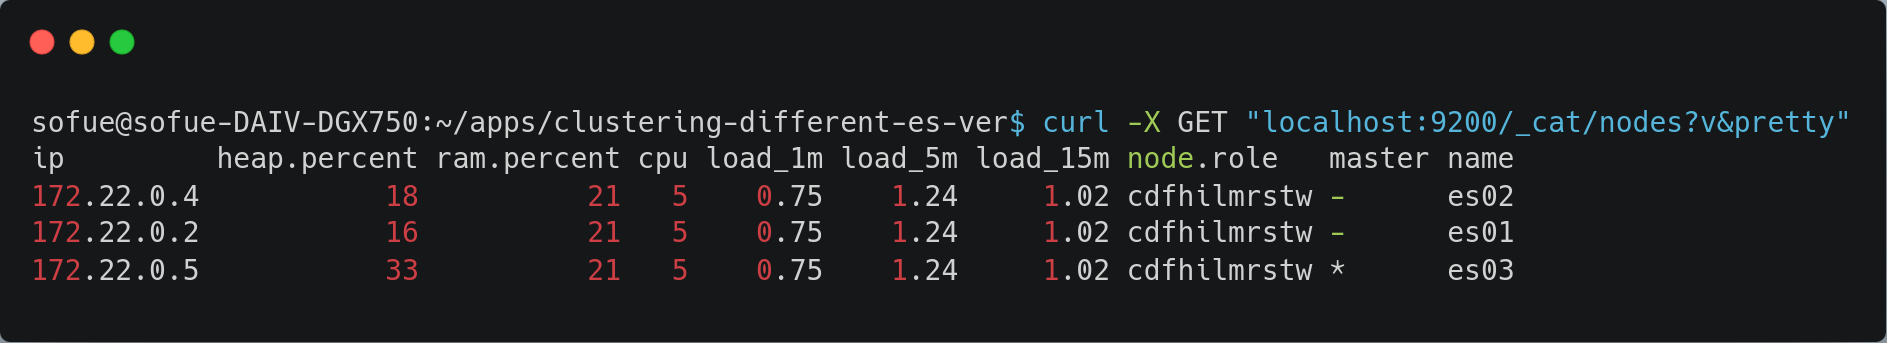
\includegraphics[width=140mm]{sotu/figure/4nodes-list.png}
%     \caption{クラスタに参加しているノード一覧}
%     \label{4-p14}
%   \end{center}
% \end{figure}
\begin{lstlisting}[language=bash, caption=クラスタBに参加しているノード一覧, label=4-sc7]
  $ curl -X GET 'localhost:9200/_cat/nodes?v&pretty'
  ip         heap.percent ram.percent cpu load_1m load_5m load_15m node.role   master name
  172.30.0.4           22          88  28    5.99    2.99     1.72 cdfhilmrstw -      es03
  172.30.0.3           17          88  29    5.99    2.99     1.72 cdfhilmrstw *      es02
  172.30.0.2           36          88  30    5.99    2.99     1.72 cdfhilmrstw -      es01
\end{lstlisting}

リスト \ref{4-sc7}より, クラスタAのノードがクラスタBに参加できていないことを確認した.

es04コンテナ(クラスタAに参加しているノード)で出力されたログの一部をリスト \ref{4-sc8}に示す.

% \begin{figure}[H]
%   \begin{center}
%     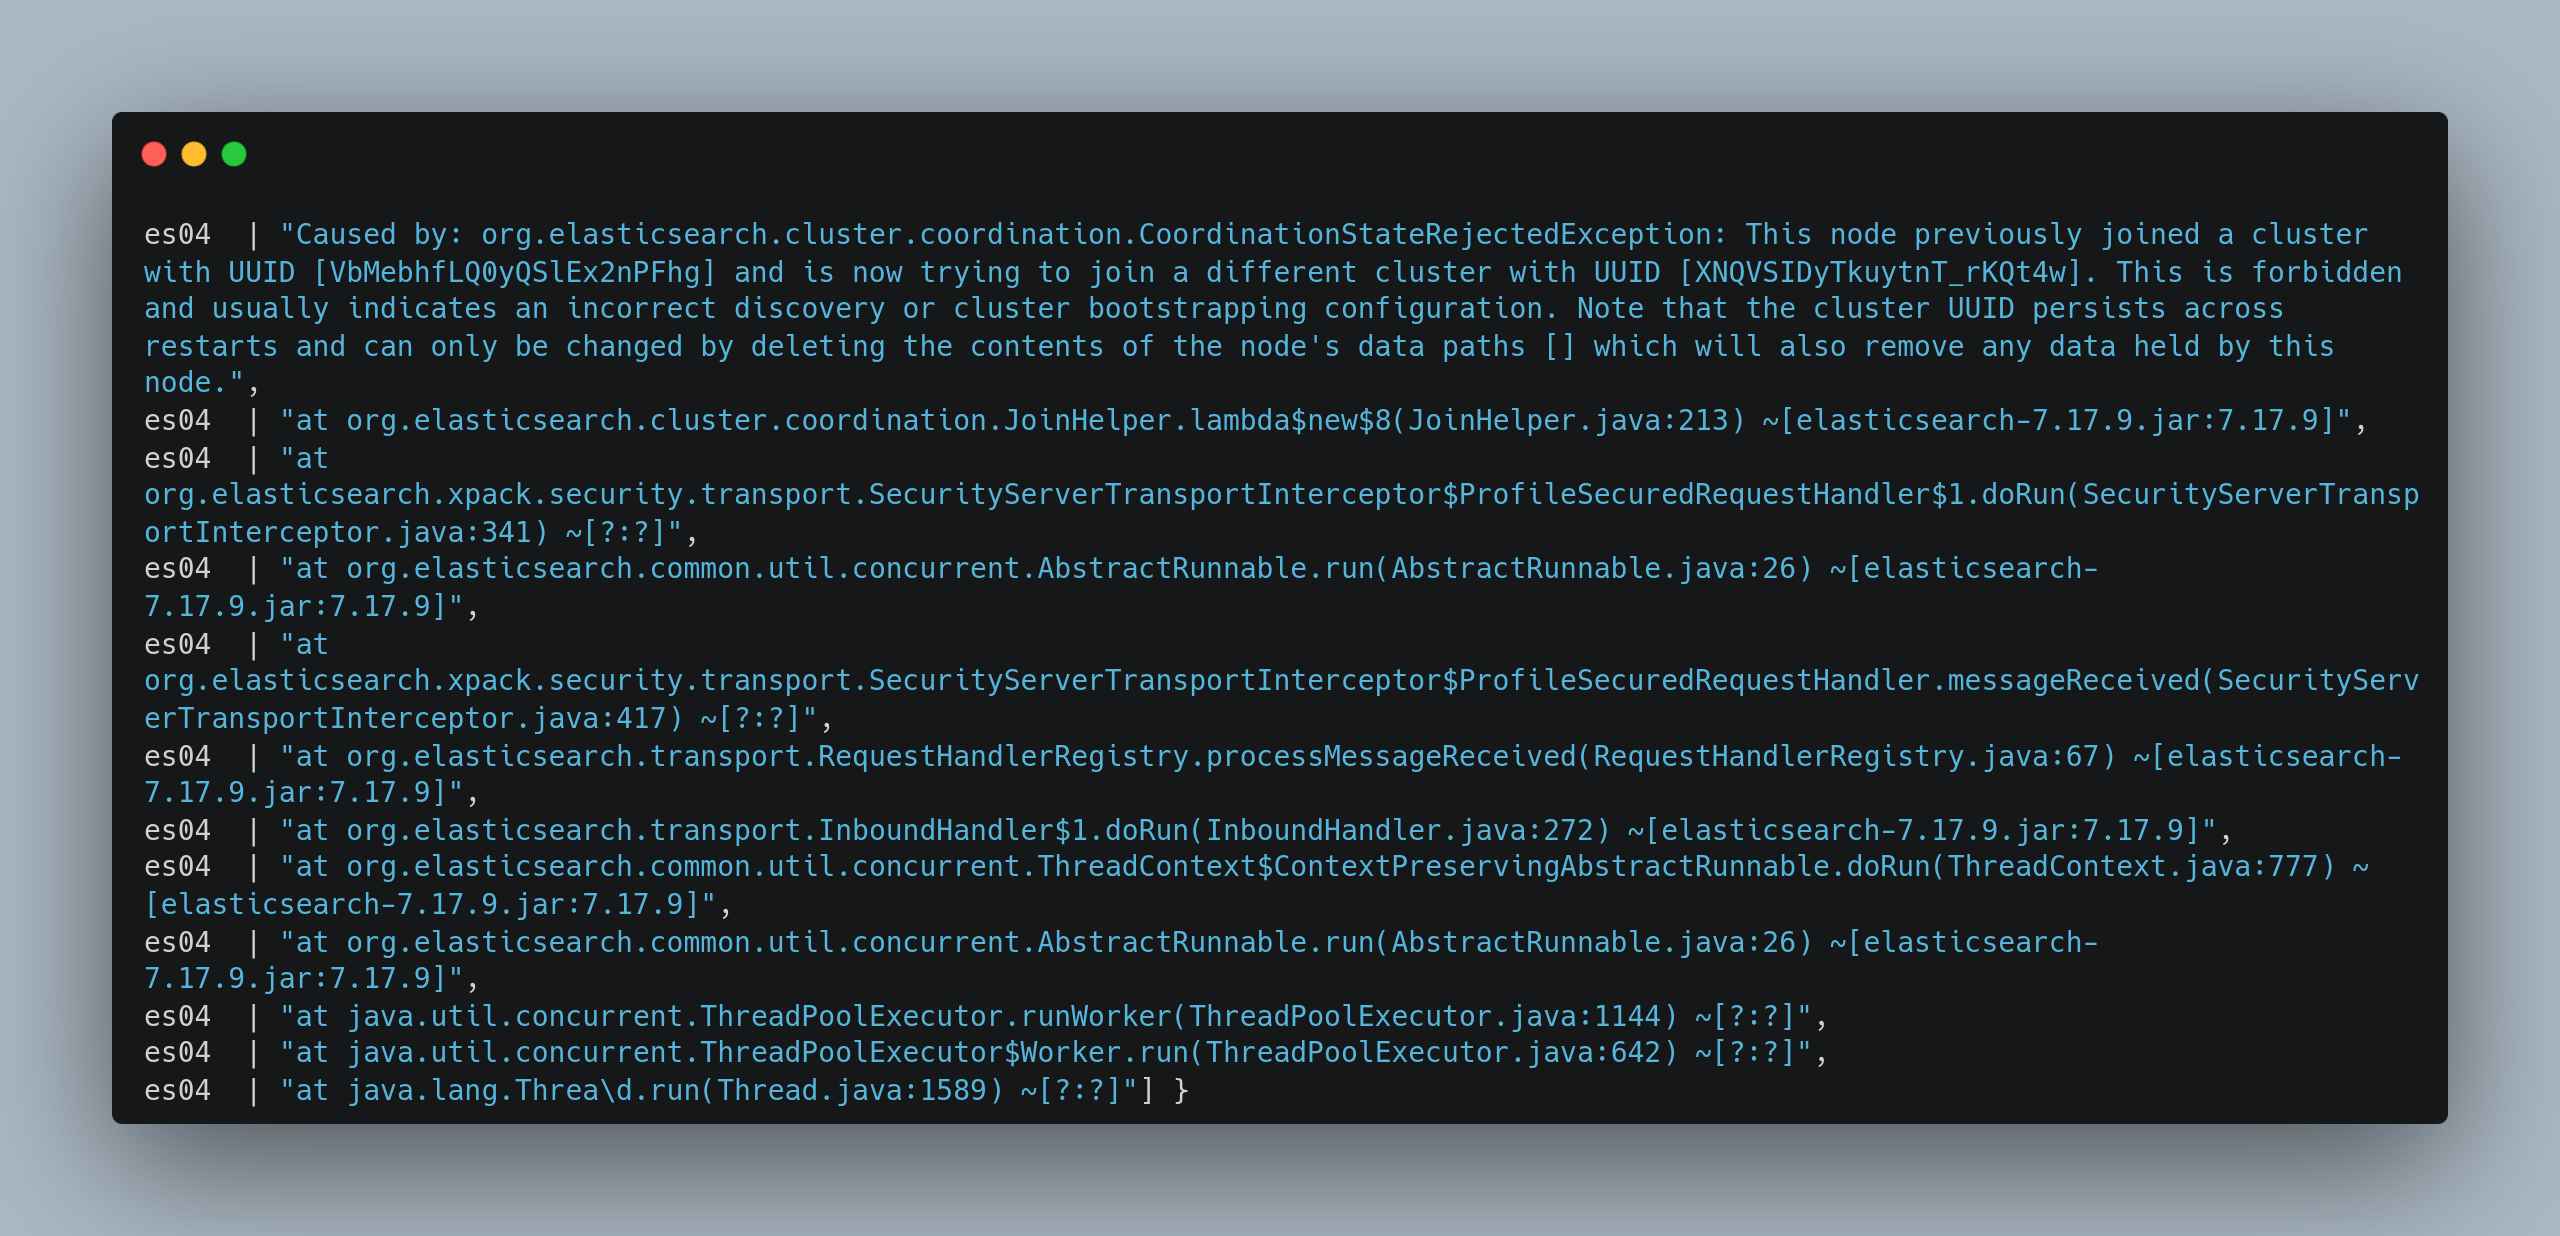
\includegraphics[width=140mm]{sotu/figure/es04-log.png}
%     \caption{es04コンテナのログの一部}
%     \label{4-p15}
%   \end{center}
% \end{figure}
\begin{lstlisting}[language=bash, caption=es04コンテナのログの一部, label=4-sc8]
This node previously joined a cluster with UUID
[2A69V1hxSFCisgmIo1LB_A] and is now trying to join a different
cluster with UUID [NCg_UaW0Q6KTakJG5HJrHg].
This is forbidden and usually indicates an incorrect discovery
or cluster bootstrapping configuration. Note that the cluster
UUID persists across restarts and can only be changed by
deleting the contents of the node's data paths [] which will
also remove any data held by this node.
\end{lstlisting}

リスト \ref{4-sc8}では, 異なるクラスタIDを持つクラスタにノードが参加することは禁止されており, 参加するためにはインデックスやドキュメント情報などが格納されているデータパス配下のフォルダ, ファイルを削除する必要があると書かれている.

以上の検証結果から, 既に稼働しているノードを別のクラスタに新しいノードとして参加させることは出来ないことが分かった.

\section{結言}
本章では, 異なるバージョンのElasticsearchノードを用いたクラスタリングの動作の検証と, 異なるクラスタへの Elasticsearchノードの参加の可否の検証を行った.

はじめに, 異なるバージョンのElasticsearchノードのクラスタリングを検証した. まず同じバージョンのElasticsearchノードを用いてクラスタを構築した後, 異なるバージョンの Elasticsearchノードを新たにクラスタに含めてクラスタ起動を試みたが, バージョンの不一致によりクラスタリングは失敗した. これにより, 異なるバージョンのElasticsearchノードを用いたクラスタ構築は出来ないことを確認した.

次に, 既に稼働している Elasticsearchノードを異なるクラスタに参加させる検証を行った. まずクラスタAとクラスタBをそれぞれ構築した後, クラスタAの ElasticsearchノードをクラスタBの Elasticsearchノードとして参加させて, クラスタBの起動を試みた. しかし, クラスタAの ElasticsearchノードはクラスタBに参加できなかった. これにより, 既に稼働している Elasticsearchノードを異なるクラスタに参加させることは出来ないことを確認した.

\begin{figure}[H]
  \begin{center}
    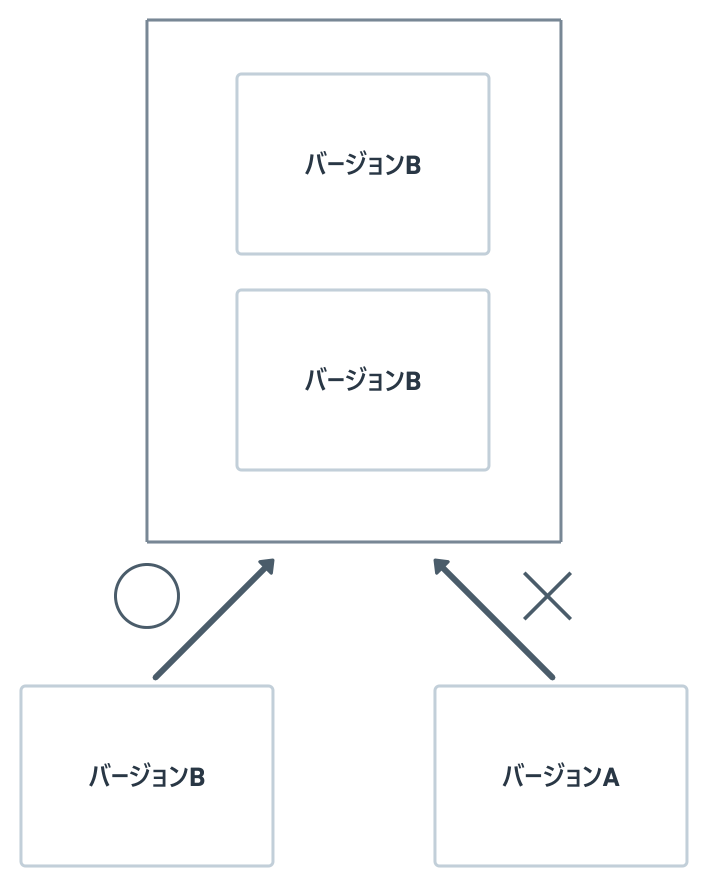
\includegraphics[width=120mm]{sotu/figure/youshi-3.png}
    \caption{Elasticsearchノードのバージョンが異なる場合のクラスタリングの可否}
    \label{4-p16}
  \end{center}
\end{figure}

\begin{figure}[H]
  \begin{center}
    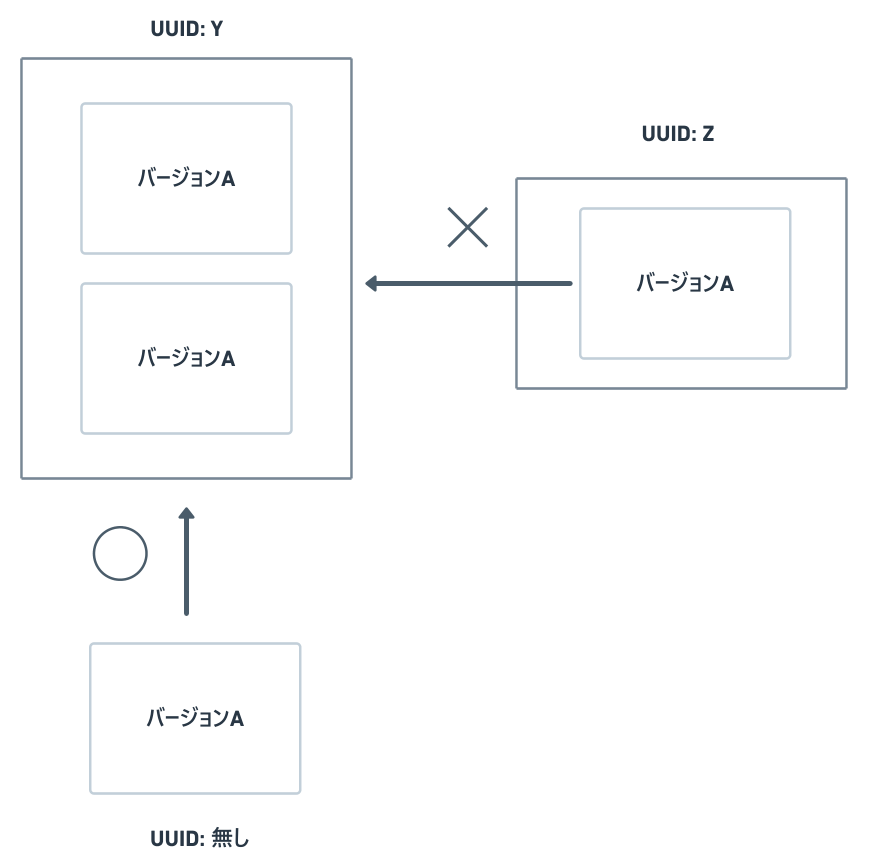
\includegraphics[width=120mm]{sotu/figure/youshi-4.png}
    \caption{UUIDが異なるクラスタにElasticsearchノードを参加させた場合のクラスタリング動作の可否}
    \label{4-p17}
  \end{center}
\end{figure}

次章では結論と今後の課題について述べる.
